% to render
% pdflatex [ filename ] && pdflatex [ filename ]

\documentclass{article}
% \documentclass[twocolumn]{article}

\usepackage{graphicx}
\usepackage{amsmath, amsthm, amssymb}
\usepackage{parskip}

% block code
\usepackage{alltt}

% set margins
\usepackage[margin = 1in]{geometry}
\setlength{\parindent}{1cm}

\usepackage{setspace}
% for double spacing the entire document
% \doublespacing
\singlespacing

% fancier captions
\usepackage{caption}
\captionsetup[figure]{font = small, labelfont = small}

%% imported packages
\usepackage{paralist}

% reference tables and figures, in the style of eqref
\newcommand{\figref}[1]{Fig. (\ref{#1})}
\newcommand{\tabref}[1]{Table (\ref{#1})}

% stylistic shortenings
\newcommand{\ti}[1]{\emph{#1}}
\newcommand{\tb}[1]{\textbf{#1}}
\newcommand{\cpart}[1]{\newblock{\LARGE {\\\\#1}}}
\renewcommand{\arraystretch}{1.3}

% comments that should be hidden
\newcommand{\comment}[1]{}

% note syntax
\newcommand{\note}[1]{\newblock{\small [ \ti{\tb{#1}} ]}}
% hide notes
% \newcommand{\note}[1]{\comment{#1}}

% inline code
\newcommand{\code}[1]{\texttt{$\text{#1}$}}

% vector stylization
\newcommand{\vect}[1]{\boldsymbol{#1}}
% \newcommand{\vect}[1]{\vec{#1}}

\begin{document}
% small text
% \small

\title{\tb{Parallel Floyd-Warshall Performance}}
\author{Minke Zhang\hspace*{-\tabcolsep}}
\date{\today}

% make title
\begingroup
\let\center\flushright
\let\endcenter\endflushright
\maketitle
\endgroup

\section{Design Document}
\cpart{Modules}

As per the requirements documentation, we shall split the Floyd-Warshall implementation into three distinct parts:

	\begin{itemize}
		\item initialization,
		\item execution, and
		\item output
	\end{itemize}

We shall further roll the initialization and output modules into one "io" module (cf. \code{io.h}). The high-level purpose of the module is to provide an easy way 
for data to be read and written to external files; specifically, we shall expose the following methods to the user:

\begin{alltt}
int **read_array(char *arr, int *dim);
void write_array(char *fn, int dim, int **arr);
\end{alltt}

The execution module (cf. \code{fw.h}) is where the bulk of the execution resides -- we wish to pass into the module the array (graph) to be processed, and have as 
output the result of the algorithm -- that is an array such that \code{arr[i][j]} represents the minimal weight of the path between \code{i} and \code{j}. We shall 
expose the following methods to the user:

\begin{alltt}
void execute_serial(int dim, int **arr);
void execute_parallel(int dim, int **arr, int thread_count);
\end{alltt}

Additionally, for testing purposes we have exposed

\begin{alltt}
void execute(int i, int j, int k, int **arr);
\end{alltt}

though it is understood that the user shall not use this method directly within the algorithm execution.

\cpart{Algorithm Overview}

From Wikipedia, we have the pseudocode for the Floyd-Warshall algorithm:
\begin{alltt}
for k from 1 to |V|
  for i from 1 to |V|
    for j from 1 to |V|
      if dist[i][j] > dist[i][k] + dist[k][j]
         dist[i][j] = dist[i][k] + dist[k][j]
       end if
\end{alltt}

It is clear here that the algorithm runs in $\mathcal{O}(|V|^3)$ time; however, though practically speaking this is a computationally solvable problem, $n^3$ time 
is still at times rather infeasible. We would therefore like to see if there is a way to speed up the algorithm, while at the same time committing a minimal amount 
of work for this speedup -- we wish to implement a parallel version of the algorithm, which in ideal cases, will give an $m \times$ speedup given $m$ cores. Here, 
rather than attempting to manufacture an arbitrary number of cores, we shall instead analyze the case in which the algorithm is executed in parallel with respect to 
an arbitrary number of \ti{threads}.

\cpart{Parallel Implementation}

We see both here, as well as on the Wikipedia article, that the Floyd-Warshall algorithm is iterative on $k$, which is to say we cannot parallelize the outer loop. 
The remaining problem then is to see how to successfully split the calculation of the remaining two loops among the $m$ threads.

We will define \code{arr[i][j]} to be the $j^\text{th}$ element of the 
$i^\text{th}$ row in the array \code{arr}. Consider some array $A$ with current 
indices $k = 2$, $i = 2$, $j = 4$:

$$
\begin{array}{ccccccc}
& 1 & 2 & 3 & 4 & ... & N \\
1 & 0 & a & b & c & \cdots & d \\
2 & a & 0 & e & \tb{f} & \cdots & g \\
3 & b & e & 0 & h & \cdots & i \\
4 & c & f & h & 0 & \cdots & j \\

\vdots & \vdots & \vdots & \vdots & \vdots & \ddots & \vdots \\

N & d & g & i & j & \cdots & 0
\end{array}
$$

Where $\tb{f} == \code{A[i][j]}$, $0 == \code{A[i][k]}$, and $f == \code{A[k][j]}$. Note that, as $A$ physically represent the weighted distance between nodes, 
$\text{dist}(i, j) == \text{dist}(j, i)$, which is to say that $A$ is symmetric about the diagonal. Furthermore, note that according to the Floyd-Warshall 
algorithm, the $k^\text{th}$ row (the same as the $k^\text{th}$ column) remains \ti{unchanged} for the duration of the $k^\text{th}$ iteration, and the results of 
the calculation is \ti{only} based on this row and column. Thus, each calculation is $\ti{completely}$ independent.

If we choose to do so, we can further optimize the Floyd-Warshall algorithm by looping over $j > i$ in the inner loop; for large $N$, this will cut the number of 
comparison loops in half, which is certainly an impressive speedup. However, for at least the first parallel implementation, we will loop over the entire array, and 
focus on finding the number of threads which will balance thread overhead and thread speedup for optimal processing time.

The simplest parallel implementation of the Floyd-Warshall algorithm then would simply split the array $A$ into (a configurable number of) rows; while issues of 
load balance may become evident in other cases, the Floyd-Warshall algorithm is very predictable in memory access patterns and execution time -- thus, we shall use 
this simple implementation for the purposes of our testing.

Each thread will need to keep track of the global array to be accessed -- thus, we will employ a \code{blob} object which will be passed to all threads (cf. fw.c):

\begin{alltt}
struct blob \{
  int * **arr_addr;
  int dim;
  pthread_barrier_t fence;
  int thread_count;
\};
\end{alltt}

For the sake of ensuring \code{k} is strictly monotonic in the execution of our algorithm, we shall employ a pthread mutex structure to wait for all threads to 
finish calculating a particular value of \code{k} before moving on. As mentioned previously, as each \code{[i][j]} element can be calculated independently of one 
another, there is no need for a lock to ensure:

\begin{itemize}
	\item Each element is modified by one thread at a time, or
	\item Each element is calculated once and only once
\end{itemize}

Furthermore, as we are splitting the algorithm in a static manner, we shall be able to avoid these issues in any case.

Each thread will also privately need to keep track of its starting and end row:

\begin{alltt}
struct thread_data \{
        int tid;
        int cur_row;			// starting row
        int end_row;			// ending row -- will NOT calculate this row
        struct blob *shared_data;	// 
\};
\end{alltt}

\cpart{Testing}

We shall test several key features of the program:

\begin{itemize}
	\item Input fails gracefully on bad files
	\item Output will successfully write an array to file
	\item \code{execute()} behaves as expected
	\item \code{execute\_serial()} and \code{execute\_parallel()} will modify \code{int **arr} in the same manner
\end{itemize}

To do this, we have defined a testing framework (cf. \code{test.c}). Each test is spawned as a thread, and will exit with the appropriate exit code (either 
\code{SUCCESS} or some error code defined in \code{config.h}). These are checked against the expected return code which was set in the thread data structure. The 
main testing suite (\code{test\_all()}) will return \code{ERROR} if any of the tests failed.

\section{Hypotheses}

When executing the parallel version of the Floyd-Warshall algorithm with one thread spawned, we expect some overhead costs, for the fact that there is simply more 
lines of code physically written for the parallel case which is not handled by the serial case. Thus, for small-sized arrays where the main time of the program is 
not in the loop, we expect to see a significant overhead evident. The array size at which this overhead becomes relatively negligable we shall denote 
$N_\text{crit}$.

For multiple threads then, we expect that as long as \ti{each} thread handles $N_\text{crit}$ rows, the speedup from multiple threads will be significant. Past 
this, we would expect the overhead to start dominating the times spent in program execution.

\section{Results}

\cpart{Parallel Overhead}

\begin{figure}
\begin{center}
	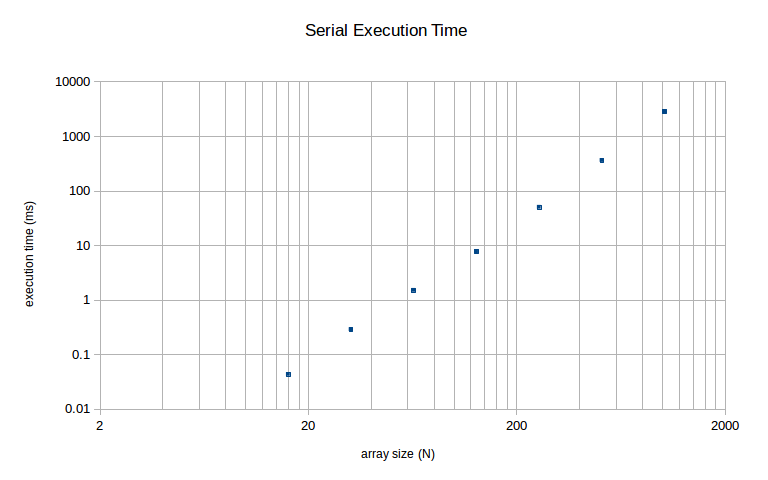
\includegraphics[scale=0.75]{serial.png}
	\caption{Serial execution time as a function of array size. Each data point is averaged over ten samples.}
	\label{serial}
\end{center}
\end{figure}

\begin{figure}
\begin{center}
	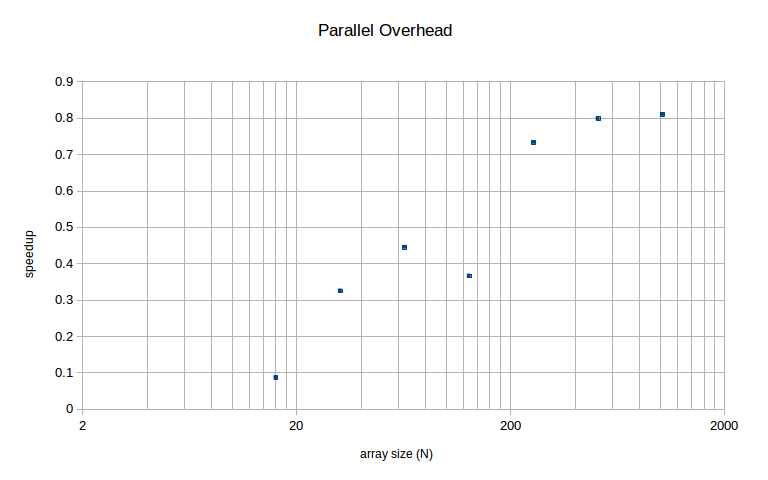
\includegraphics[scale=0.75]{overhead.png}
	\caption{Relative speedup as a function of array size of the parallel implementation in units of serial execution time. Each data point is averaged over ten samples.}
	\label{overhead}
\end{center}
\end{figure}

We see that as expected, the general overhead decreases as $N$ increases -- at $N = 1024$, the overhead costs the parallel implementation 10\% running time, though 
at $N = 16$, there is a 90\% overhead penalty. We also see a feature in \figref{overhead} at $N = 128$, such that the speedup trend dips back down to 
$\sim0.4\times$ speedup, though as seen in \figref{serial}, there are no anomalies in the serial execution time. We will make note of this when considering the 
parallel speedup results. We see that for one thread, the overall speedup passes $\sim90\%$ at $N_\text{crit} = 512$.

\cpart{Parallel Speedup}

\begin{figure}
\begin{center}
	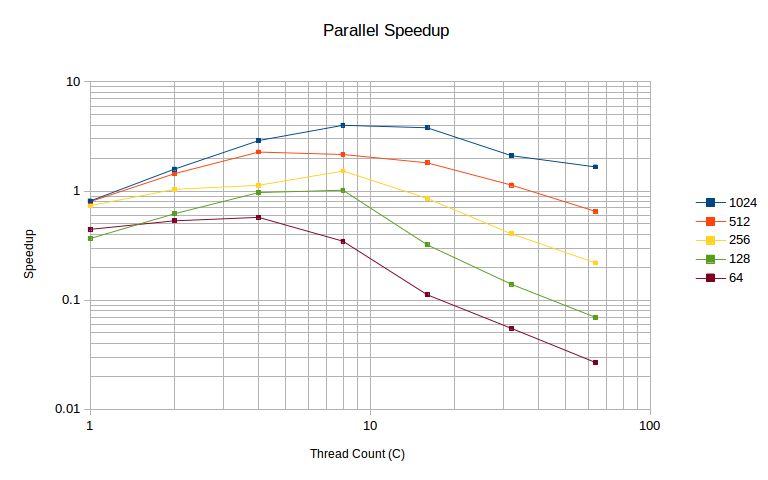
\includegraphics[scale=0.75]{speedup.png}
	\caption{Relative speedup as a function of thread count and array size as compared to the serial implementation. Each data point is averaged over ten samples.}
	\label{speedup}
\end{center}
\end{figure}

The general trend of each set of points (each differing value of $N$) is as expected -- a general increase in execution speedup, followed by the mortar shot turning 
point. We are only considering sets of points for $N > 16$ where executions across every thread count is possible.

We see that the line corresponding to $N = 128$ when measuring overhead is anomalous at $C = 1$; for more threads, we do not encounter the same behavior. As implied 
by the hypothesis, this would imply that \ti{less} time spent was spent the useful execution time (\code{execute(i, j, k, **arr)}) for the $N = 128$ than for $N = 
64$, which is clearly false. Thus, the relative slowdown must be attributed to some other factors -- it does appear that this behavior can be attributed to cache 
misses, as if this was the case, then we would expect that the slowdown rate must also be negatively impacted for all $N > 128$ as well, which does not seem to be 
the case.

We also note that the $C_\text{max}$ value at which maximal speedup occurs is not linear with respect to $N$; for $N \in \{64, 512\}$, $C_\text{max} = 4$, whereas 
for $N \in \{128, 256, 1024\}$, $C_\text{max} = 8$.

\section{Appendix}

\cpart{Directory Layout}

\begin{alltt}
./
  floyd-warshall/		// code
    code/
      results/O3.tar.gz		// code results
  writeup/			// code analysis
\end{alltt}

\end{document}
